\documentclass{article}
\usepackage[margin=2cm]{geometry}
\usepackage{amsmath, amssymb}
\usepackage{graphicx}
\usepackage{float}

% partielle ableitungen
\newcommand{\delr}{\partial_r}
\newcommand{\deltheta}{\partial_\theta}
\newcommand{\delphi}{\partial_\varphi}

% elektrische feldkonstante
\newcommand{\epsz}{\epsilon_0}

\begin{document}
\section*{Aufgabe 2}
\paragraph{a)}
$\Delta$ in Kugelkoordinaten:
\[
	\Delta f = \frac 1 {r^2}(
	\delr ( r^2 \delr f) +
	\frac 1 {\sin\theta} \deltheta (\sin\theta \deltheta f) +
	\frac 1 {\sin^2\theta} \delphi^2f)
\]
Die Poisson-Gleichung lautet:
\[
	\Delta \phi(r,\theta,\varphi) = \frac{-\rho(r,\theta,\varphi)}
	{\epsilon_0}
\]
Da die Ladung als Kugel (also symmetrisch zu $\theta$ und $\varphi$)
angeordnet ist, vereinfacht sich diese:
\[
	\Delta \phi(r) = \frac{-\rho(r)}{\epsilon_0}
\]
Die partiellen Ableitungen zu $\theta$ und $\varphi$ sind dem ensprechend
auch 0. \\
Durch zweifaches Integrieren können wir für $r > R$ ermitteln:
\begin{align*}
	\Delta \phi =
	\frac 1 {r^2} \delr \left(r^2 \delr \phi \right)
	&= \frac{- \rho_0}{\epsz} = 0\\
	\Leftrightarrow
	\delr \left( r^2 \delr \phi \right) &= 0 \\
	\Leftrightarrow
	r^2 \delr \phi  &= \alpha \\
	\Leftrightarrow
	\delr \phi  &= \frac{\alpha}{r^2} \\
	\Leftrightarrow
	\phi  &= -\frac{\alpha}{r} + \beta\\
\end{align*}
Ebenso kann man für $r \leq R$ ermitteln:
\begin{align*}
	\Delta \phi =
	\frac 1 {r^2} \delr \left(r^2 \delr \phi \right)
	&= \frac{- \rho_0}{\epsz} \\
	\Leftrightarrow
	\delr \left( r^2 \delr \phi \right)
	&= \frac{- \rho_0 }{\epsz} r^2  \\
	\Leftrightarrow
	r^2 \delr \phi
	&= \frac{- \rho_0 }{3  \epsz} r^3 + \gamma \\
	\Leftrightarrow
	\delr \phi
	&= \frac{- \rho_0 }{3  \epsz} r + \frac \gamma {r^2} \\
	\Leftrightarrow
	\phi
	&= \frac{- \rho_0 }{6  \epsz} r^2 - \frac \gamma r + \delta \\
\end{align*}
\paragraph{b)}
\par{1.}
Für die erste RB $-\infty < \lim_{r\rightarrow 0} \phi(r) < \infty$ muss
gelten:
\[
	\lim_{r\rightarrow 0} \phi(r) = \lim_{r\rightarrow 0}
	\frac{- \rho_0 }{6  \epsz} r^3 - \frac \gamma r + \delta
	\overset{!}{\in} (-\infty, \infty)
	\Rightarrow
	\gamma = 0
\]
\par{2.}
Die Bedingung, dass das Potential für $r \rightarrow \infty$ gegen 0 gehen
soll bewirkt, dass die Werte des Potentials auf einen festen Wert gesetzt werden. \\
Ohne diese könnte man durch $\beta$ und $\delta$ das Potential beliebig nach
oben und unten Verschieben. Einen Punkt im Unendlichen als Referenz zu
wählen, ist jedoch die Konvention in der Physik.
\[
	\lim_{r \rightarrow \infty} \phi(r) = \lim_{r \rightarrow \infty}
	-\frac{\alpha}{r} + \beta = \beta \overset{!}{=} 0
	\Rightarrow \beta = 0
\]
Damit folgt das Potential $\phi(r)$ und die Ableitung $\phi^\prime(r)$:
\[
	\phi(r) =
	\begin{cases}
		-\frac \alpha r & \text{falls } r > R \\
		-\frac{\rho_0}{6\epsz} r^2 + \delta
		& \text{falls } r \leq R
	\end{cases}
	\qquad
	\phi^\prime(r) =
	\begin{cases}
		\frac\alpha{r^2}
		& \text{falls } r > R \\
		-\frac{\rho_0}{3\epsz} r
		& \text{falls } r \leq R
	\end{cases}
\]
\newpage
\par{3.}




\newpage
\section*{Aufgabe 3}
Die Ladungsdichte der Elektronen war gegeben durch
\[
	\rho_e(\vec r) = - \frac{e}{\pi a^3} \exp\left(-\frac{2r}{a} \right)
\]
Damit folgt das elektrische Potential, welches durch das Elektron erzeugt
wird:
\begin{align*}
	\phi_e\left( \vec r \right)
	&= \frac 1 {4\pi\epsz}
	\int_0^\infty \int_0^\pi \int_0^{2\pi}
	\frac{\rho_e(\vec r^\prime) r^{\prime 2} \sin\vartheta^\prime}
	{d \left(\vec{r^\prime}, \vec r \right) }
	d\varphi^\prime d\vartheta^\prime dr^\prime \\
	% rho einsetzen
	&= \frac 1 {4\pi\epsz}
	\int_0^\infty \int_0^\pi \int_0^{2\pi}
	\frac{
	- \frac{e}{\pi a^3} \exp\left(-\frac{2r^\prime}{a} \right)
	r^{\prime 2} \sin\vartheta^\prime}
	{d \left(\vec{r^\prime}, \vec r \right) }
	d\varphi^\prime d\vartheta^\prime dr^\prime \\
	% nach phi integrieren
	% d einsetzen
	% linearitaet des integrals
	&= - \frac e {2 a^3 \pi\epsz}
	\int_0^\infty \int_0^\pi
	\frac{
	 \exp\left(-\frac{2r^\prime}{a} \right)
	r^{\prime 2} \sin\vartheta^\prime}
	{\sqrt{r^2 + r^{\prime 2} + 2r r^\prime \cos\theta^\prime}}
	d\vartheta^\prime dr^\prime \\
	% nach theta integrieren
	&= - \frac e {2 a^3 \pi\epsz}
	\int_0^\infty
	\exp\left(-\frac{2r^\prime}{a} \right)
	\frac{r^\prime}{r} \underbrace{ \left(
	\sqrt{r^2 + r^{\prime 2} + 2r r^\prime} -
	\sqrt{r^2 + r^{\prime 2} - 2r r^\prime} \right)}_{
		\xi :=}
	dr^\prime \\
\end{align*}
Mit einer Fallunterscheidung lässt sich $\xi$ durch Verwendung der
binomischen Formeln vereinfachen:
\begin{align*}
	r &> r^\prime: &
	\xi &= \sqrt{(r + r^\prime)^2} - \sqrt{(r - r^\prime)^2}
	= (r + r^\prime) - (r - r^\prime) = 2r^\prime \\
	r &< r^\prime: &
	\xi  &= \sqrt{(r^\prime + r)^2} - \sqrt{(r^\prime - r)^2}
	= (r^\prime + r) - (r^\prime - r) = 2r
\end{align*}
Da für $\xi$ 2 Fälle existieren Teilen wir das Integral an dieser Stelle
auf.\\
Durch partielle Integration erhalten wir dann:
\begin{align*}
	\phi_e\left( \vec r \right)
	&= - \frac{e}{r a^3 \pi\epsz}
	\int_0^r
	\exp\left(-\frac{2r^\prime}{a} \right)
	r^{\prime 2}
	dr^\prime
	- \frac e {a^3 \pi\epsz}
	\int_r^\infty
	\exp\left(-\frac{2r}{a} \right)
	r^\prime \
	dr^\prime
	\\
	% integral loesen
	&= - \frac{e}{r a^3 \pi\epsz}
	\left[
		\exp\left(\frac{-2r^\prime}{a}\right)
		\left( \frac{-r^{\prime 2}a}{2} - \frac{r^\prime a^2}{2} - 
		\frac{a^3}{4}
		\right)
		+\frac{a^3}{4}
	\right]_0^r 
	- \frac e {a^3 \pi\epsz}
	\left[
		\exp\left(\frac{-2r^\prime}{a}\right)
		\left( \frac{r^\prime a}{2} + \frac{a^2}{4} \right)
	\right]_r^\infty
	\\
	% einsetzen in stammfkt
	&= - \frac{e}{r a^3 \pi\epsz}
		\exp\left( \frac{-2r}{a} \right) *
		\left(
		\frac{-r^2a}{2} - \frac{ra^2}{2} - \frac{a^3}{4}
		\right)
	- \frac{e}{r a^3 \pi\epsz}
		\frac{a^3}{4}
	- \frac{e}{a^3 \pi \epsz}
	\left[
		\exp\left( \frac{-2r}{a} \right) * 
		\left(
		\frac{ra}{2} + \frac{a^2}{4}
		\right)
	\right]
	% vereinfachen
\end{align*}


\section*{Aufgabe 4}
\paragraph{a)}
\begin{align*}
	\phi(\vec r) 
	&= \frac{1}{4\pi\epsz} \int \frac{\rho(\vec r)}{\vert \vec r - \vec{
		r^\prime} \vert} d^3 \vec r^\prime \\
	% rho einsetzen
	% distanz einsetzen
	&= \frac{1}{4\pi\epsz} 
		\int_0^\pi \int_0^{2\pi} \int_0^\infty
		\frac{
		\sigma_0 \cdot \delta(r^\prime - R) \cdot \Theta
		\left( \vartheta - \frac \pi 2 \right)}
		{\sqrt{ r^2 + r^{\prime 2} + 2 r r^\prime \cos\vartheta }}
		r^{\prime 2} \sin\vartheta \
		dr^\prime d\varphi d\vartheta \\
	% delta funktion auswerten
	% rprime muss durch R ersetzt werden
	&= \frac{1}{4\pi\epsz} 
		\int_0^\pi \int_0^{2\pi}
		\frac{
		\sigma_0 \cdot \Theta 
		\left( \vartheta - \frac \pi 2 \right)}
		{\sqrt{ r^2  + R^2 + 2 r R \cos\vartheta }}
		R^2 \sin\vartheta \
		d\varphi d\vartheta \\
	% heaviside auswerten 
	% theta grenzen verschiheben sich
	&= \frac{1}{4\pi\epsz} \cdot 2\pi
		\int_{\frac \pi 2}^{\pi}
		\frac{\sigma_0 \cdot R^2 \sin\vartheta}
		{\sqrt{ r^2  + R^2 + 2 r R \cos\vartheta }}
		d\varphi \\
	% theta integrieren
	&= \frac{1}{2\epsz} \sigma_0 \frac{R 
	\sqrt{R^2 + r^2 - 2rR\cos\vartheta}}{r} 
	|_{\frac \pi 2}^\pi \\
	% theta einsetzen
	&= \frac{R \cdot \sigma_0}{2 r \epsz} \left(
		\sqrt{R^2 + r^2 + 2rR} - \sqrt{R^2 + r^2}
	\right) \\
	% binomiosches formel
	&= \frac{R \cdot \sigma_0}{2 r \epsz} \left(
		R + r - \sqrt{R^2 + r^2}
	\right) \\
\end{align*}

\paragraph{b)}
\mbox{}
\begin{figure}[H]
	\centering
	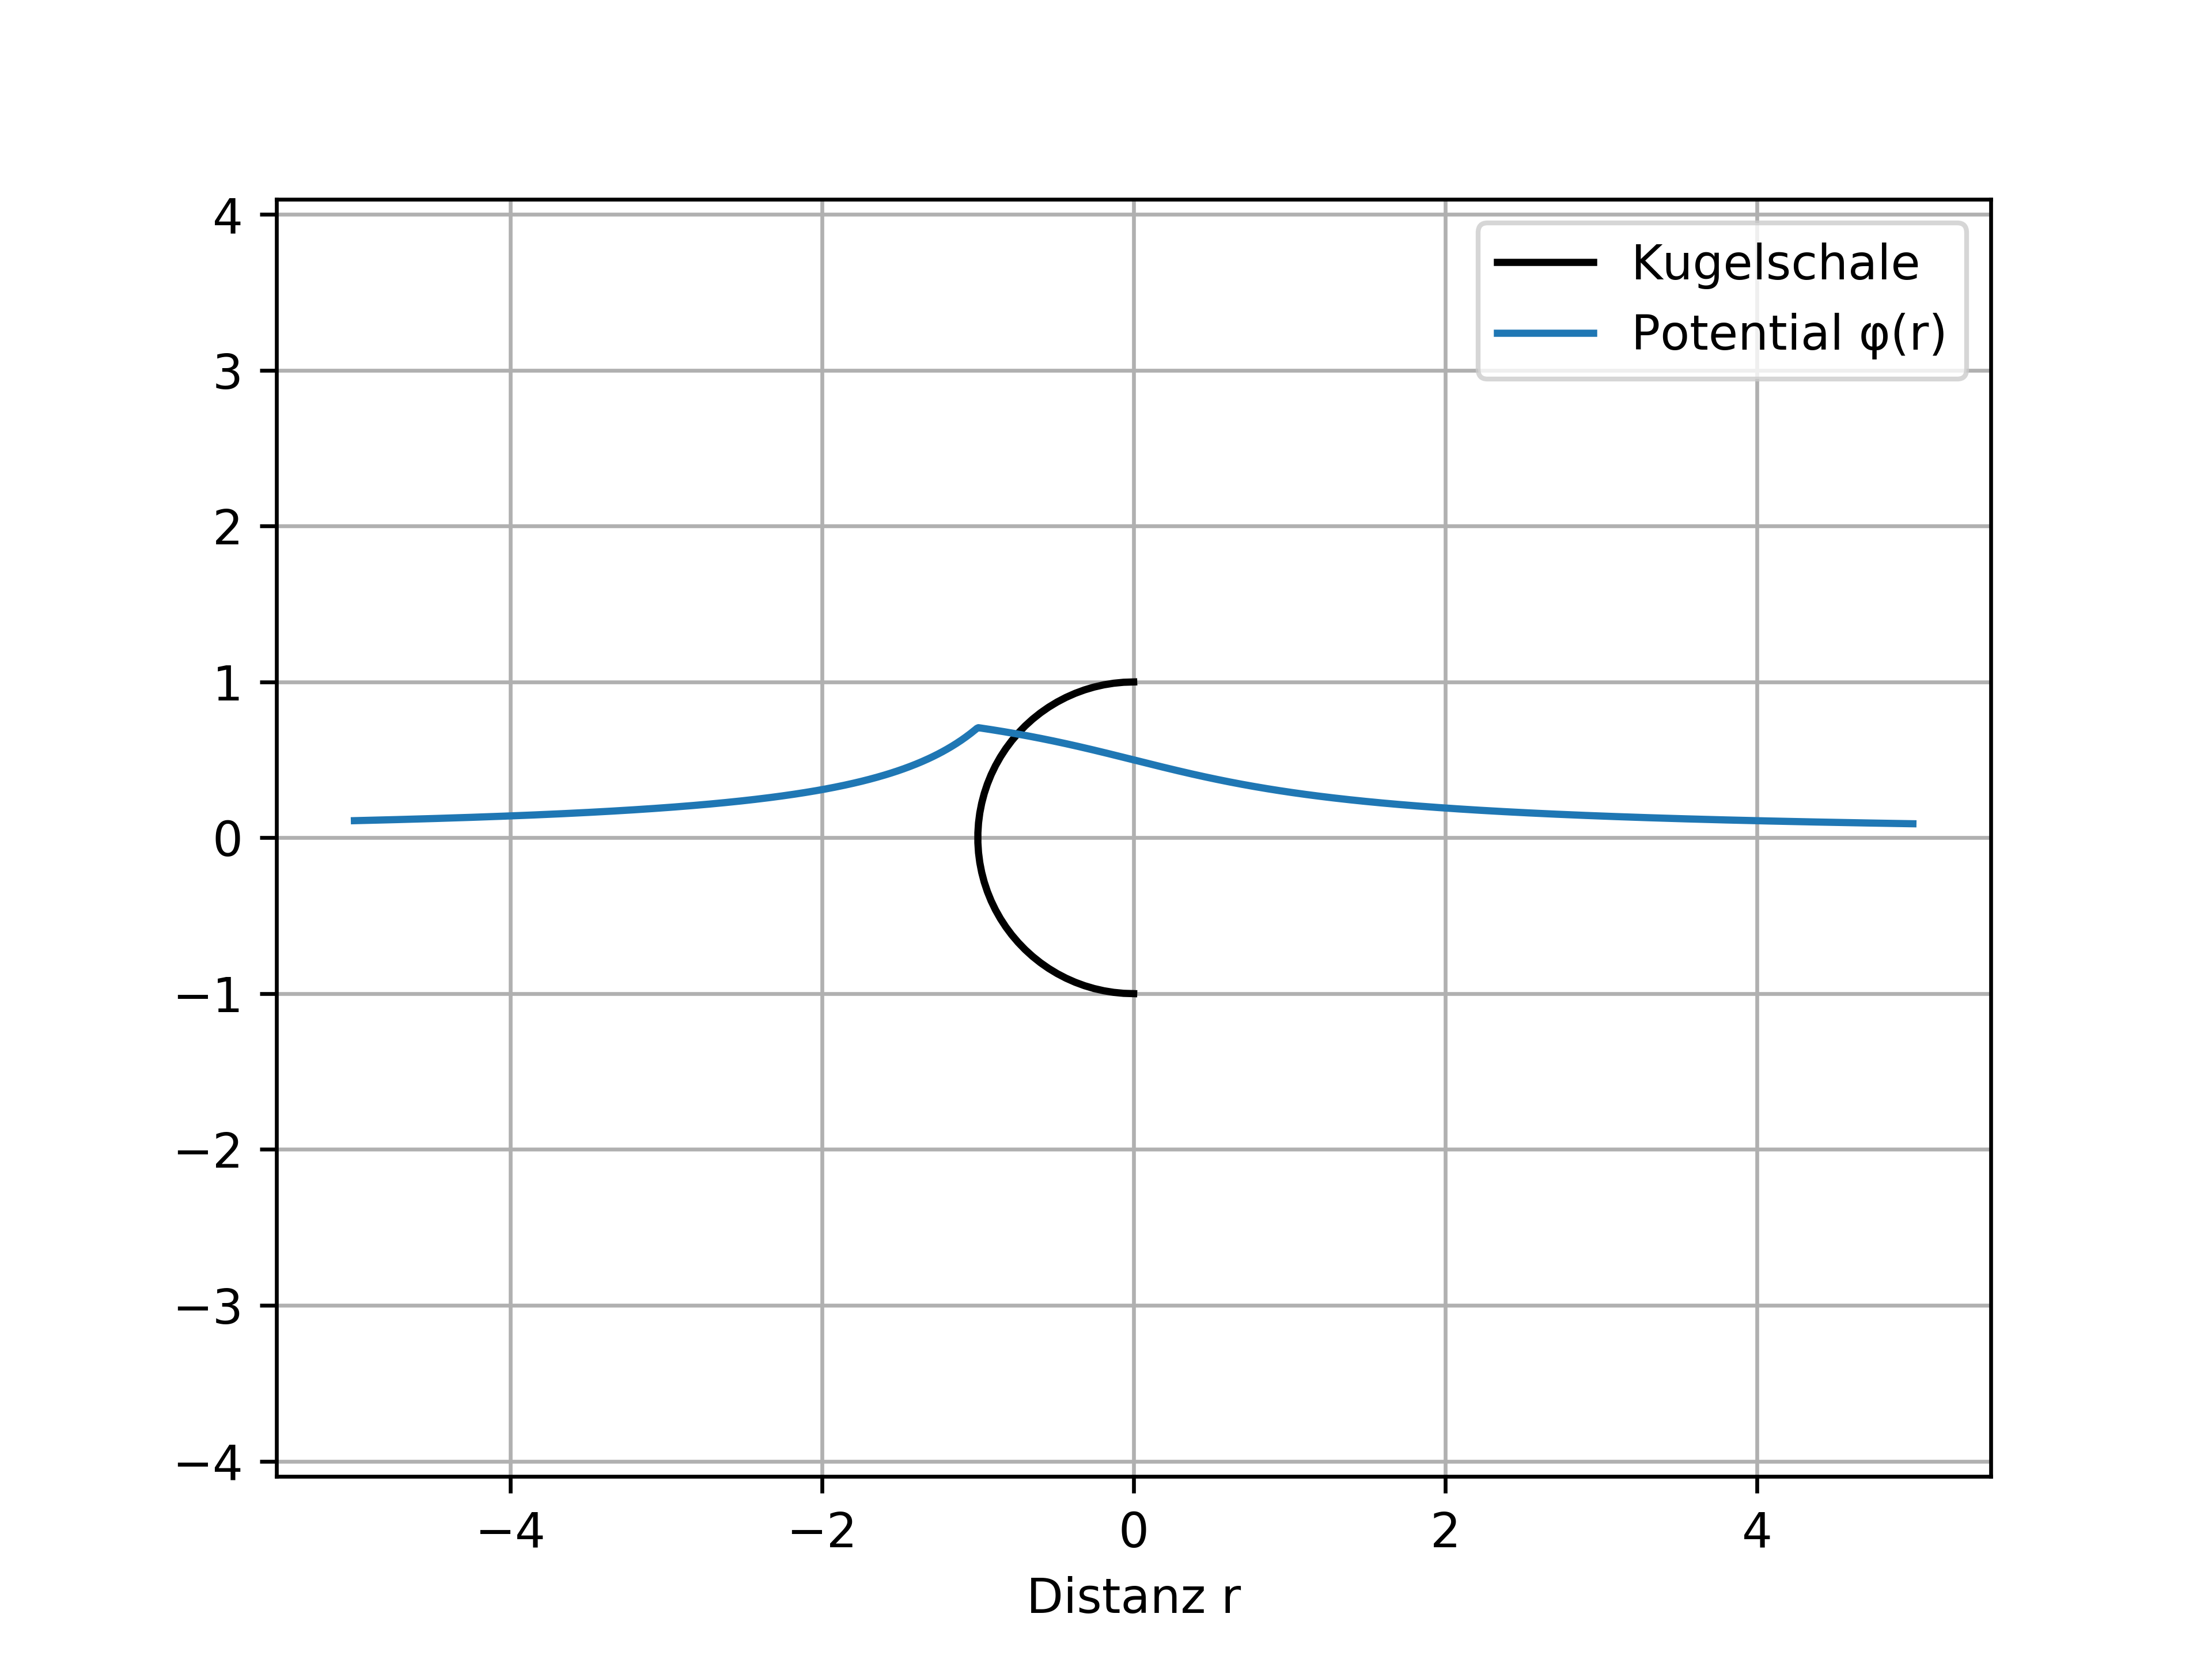
\includegraphics[width=15cm]{aufgabe4plot.png}
\end{figure}

\newpage
\section*{Aufgabe 5}
\par{a)}
\[
	\int_{-2}^5 \underbrace{(x^2 - 5x + 6)}_{f(x) :=}
	\delta(x-3) dx
	= f(3) = 0
\]
\vspace{0.5cm}
\par{b)}
\[
	\int_\alpha^\beta
	(f(x) - f(a)) \delta(x - a) dx = 
	\begin{cases}
		f(a) - f(a)
		&\text{falls } a \in [\alpha, \beta] \\
		0
		&\text{sonst}
	\end{cases}
	= 0
	\]
\vspace{0.5cm}
\par{c)}
\[
	\int_0^\infty x^2 \delta(x^2 -3x + 2) dx
	=
	\sum_i \frac{x_i^2}{\vert 2x_i - 3 \vert} = \frac41 + \frac11 = 5
\]
$x_i$ entspricht den Nullstellen der Funktion $x^2 - 3x + 2$
\vspace{0.5cm}
\par{d)}
\[
	\int_0^\infty \ln(x) \delta^\prime(x-a) dx
	=
	\left[
		\delta(x-a) \ln(x)
	\right]_{0}^\infty
	-
	\int_0^\infty \frac1x \delta(x-a) dx
	=
	\begin{cases}
		-\infty &\text{für } a = 0\\
		-\frac1a &\text{sonst}
	\end{cases}
\]	
\vspace{0.5cm}
\par{e)}
\[
	\int_0^\pi \sin^3(\theta) \delta \left( \cos\theta - \cos\frac\pi3
	\right) dx
	=
	\frac{\sin^3 \left( \frac\pi3 \right)}
	{\vert -\sin\left( \frac\pi3 \right) \vert}
	= 
	\sin^2 \left( \frac\pi3 \right)
	= \frac34
\]


\end{document}

